%%%%%%%%%%%%%%%%%%%% MEvD-GRN ICML-STYLE PAPER %%%%%%%%%%%%%%%%%%%%
\documentclass{article}

\usepackage{microtype}
\usepackage{graphicx}
\usepackage{booktabs}
\usepackage{hyperref}
\usepackage[accepted]{icml2024}

\usepackage{amsmath}
\usepackage{amssymb}
\usepackage{mathtools}
\usepackage{amsthm}
\usepackage{algorithm}
\usepackage{algorithmic}
\usepackage{multirow}
\usepackage{xcolor}

\providecommand{\theHalgorithm}{\arabic{algorithm}}

\theoremstyle{plain}
\newtheorem{proposition}{Proposition}[section]
\theoremstyle{definition}
\newtheorem{definition}[proposition]{Definition}

\newcommand{\good}{\textcolor{green!45!black}{\checkmark}}
\newcommand{\bad}{\textcolor{red!60!black}{\ding{55}}}
\usepackage{pifont}

\icmltitlerunning{MEvD-GRN: Curriculum Learning over Confidence-Tiered Regulatory Evidence}

\begin{document}

\twocolumn[
\icmltitle{MEvD-GRN: Multi-Evidence Distillation for Gene Regulatory\\
Network Inference via Curriculum Learning over Confidence-Tiered Evidence}

\begin{icmlauthorlist}
\icmlauthor{MEvD-GRN Project}{aff}
\end{icmlauthorlist}

\icmlaffiliation{aff}{Independent research project, MEvD-GRN repository}

\icmlcorrespondingauthor{MEvD-GRN Project}{mevd-grn@example.org}

\icmlkeywords{Gene Regulatory Networks, Graph Neural Networks, Curriculum Learning, Multi-Omics, Single-Cell Genomics, Catastrophic Forgetting}

\vskip 0.3in
]

\printAffiliationsAndNotice{}

\begin{abstract}
Inferring gene regulatory networks (GRNs) -- the directed map from transcription
factors (TFs) to the target genes they control -- is a central problem in
computational biology, and single-cell multi-omic profiling (paired RNA and ATAC
sequencing) is rapidly becoming its primary data substrate. Existing reference
databases seldom acknowledge that not all regulatory edges are equally trustworthy:
an edge inferred from a TF binding assay (localization evidence) is weaker than one
inferred from a functional knockout (perturbation evidence), and edges supported by
\emph{both} are the most reliable. We introduce \textbf{MEvD-GRN}, a compact
dual-modality graph neural network that treats this confidence structure as a
training curriculum rather than as an incidental labeling detail. MEvD-GRN encodes
RNA and ATAC signals in separate towers, fuses them only at a role-aware decoder in
which chromatin accessibility gates transcriptional compatibility, and is trained
sequentially on the localization and perturbation evidence tiers of the K562 cell
line from the SC-MO-GRN-DB resource. We then evaluate the trained model in a
\emph{zero-shot} fashion on the highest-confidence dual-evidence tier -- never used
for a single gradient update -- and find that a 306,691-parameter model reaches
AUPR $0.558$ / AUROC $0.838$ on this held-out tier, exceeding a 4.08M-parameter
supervised multi-omic GNN baseline (scMultiomeGRN) and three additional classical
and deep-learning baselines. We complement this headline result with a rigorous
ablation study (10 configurations) that surfaces a genuine limitation -- sequential
curriculum training induces catastrophic forgetting of the localization tier, which
memory replay only partially remedies -- and we quantify exactly how much of the
model's competitiveness against the strongest baseline depends on the specific
curriculum schedule chosen.
\end{abstract}

\section{Introduction}
\label{sec:intro}

Every human cell shares the same genome, yet a skin cell and a neuron express
wildly different sets of genes. The switches that decide, for a given cell type,
\emph{which} genes are turned on or off are transcription factors (TFs) --
proteins that bind DNA near a target gene and either promote or repress its
expression. The full wiring diagram of ``which TF regulates which gene'' in a
given cell type is called its \textbf{gene regulatory network (GRN)}.
Reconstructing GRNs computationally from measurable molecular data is important
because it lets researchers predict the downstream effect of perturbing a single
gene, understand how cell identity is maintained or lost (e.g.\ in cancer or
reprogramming), and prioritize candidate drug targets -- all without having to
experimentally knock out every TF in every cell type, which is infeasible at
scale.

\textbf{GRN inference as link prediction.} Formally, a GRN is a directed
bipartite graph: one set of nodes is a subset of ``regulator'' genes (the TFs),
the other set is all genes in the genome, and a directed edge TF~$i \to$ gene~$j$
means TF~$i$ regulates gene~$j$. GRN inference is therefore a \textbf{link
prediction} problem, scored over a candidate space of size $|\text{TFs}| \times
|\text{genes}|$ that is enormous (millions of candidate pairs) relative to the
handful of edges that are actually true.

\textbf{Two complementary experimental measurements.} Modern single-cell
technology provides two views of a cell's regulatory state that are individually
informative but jointly more powerful: \textbf{scRNA-seq} measures which genes are
being transcribed (expression), while \textbf{scATAC-seq} measures which
stretches of DNA are physically accessible to be bound by a TF at all
(chromatin accessibility). A TF cannot regulate a gene whose locus is closed, and
a gene cannot be considered ``regulated'' in a meaningful sense if it is not also
transcriptionally responsive -- so the two modalities constrain each other
\cite{duren2018integrative}. Most GRN inference methods, however, still use only
one of the two (usually RNA alone); we build a model that treats accessibility and
expression as functionally distinct, non-interchangeable roles (Section
\ref{sec:model}).

\textbf{The overlooked structure: evidence is not created equal.} The public
database we build on, SC-MO-GRN-DB \cite{valensi2026scmogrndb}, is unusual in that
it tags every reference regulatory edge with \emph{how it was experimentally
discovered}. This produces a natural confidence hierarchy with three tiers:

\begin{itemize}
\item \textbf{Localization} edges come from TF-binding assays (ChIP-seq): high
recall (many binding events are detected) but low precision, because physical
binding does not guarantee a functional regulatory effect.
\item \textbf{Perturbation} edges come from knockdown/knockout/CRISPR
experiments: low recall (only genes that respond measurably are captured) but
high precision, since a causal expression change is direct functional evidence.
\item \textbf{Dual-evidence} edges are the intersection of the two: both a
binding event \emph{and} a functional effect are observed for the same TF-gene
pair. This is the smallest and most trustworthy tier -- the closest available
proxy to biological ground truth.
\end{itemize}

Almost every GRN inference method in the literature is agnostic to this
structure: reference networks are pooled into a single, undifferentiated set of
positive edges before training or evaluation. Our central methodological
contribution is to instead treat the tier hierarchy explicitly, as an
\textbf{evidence-tier curriculum}: train sequentially on localization then
perturbation evidence, and hold the dual-evidence tier out entirely as a
zero-shot evaluation benchmark. Section \ref{sec:curriculum} explains in detail
why this design -- rather than directly fine-tuning on the dual-evidence tier --
is the more informative test of generalization, given how the tiers are
structurally related to one another.

\textbf{Contributions.} (1) We propose MEvD-GRN, a role-aware dual-modality GNN
that keeps RNA and ATAC representations in separate encoder/GNN towers and fuses
them only through an accessibility-gated decoder (Section \ref{sec:model}). (2)
We formalize an evidence-tier curriculum with a global, hierarchy-consistent edge
splitting protocol that provides a provable guarantee against a model being
evaluated on an edge it was trained on under a different tier (Section
\ref{sec:data}), and use this guarantee to justify zero-shot evaluation of the
dual-evidence tier as the primary generalization metric (Section
\ref{sec:curriculum}). (3) We provide a rigorous empirical comparison against
four baselines -- two classical/diffusion RNA-only methods and a
4.08M-parameter supervised multi-omic GNN (scMultiomeGRN
\cite{xu2025scmultiomegrn}) -- on identical splits (Section \ref{sec:results}).
(4) We run a 10-configuration ablation study that identifies catastrophic
forgetting as the main open weakness of the sequential curriculum, quantify how
much of it memory replay recovers, and identify two alternative training
schedules (joint multi-task training and a full replay-based curriculum) that
substantially close the gap (Section \ref{sec:ablation}).

We report all results honestly, including configurations under which the
proposed model \emph{loses} to a baseline, because we believe a transparent
account of a training curriculum's failure modes is as scientifically valuable
as its successes.

\section{Related Work}
\label{sec:related}

\textbf{Classical GRN inference.} GENIE3 \cite{huynhthu2010genie3} and its
faster gradient-boosted reimplementation GRNBoost2 \cite{moerman2019grnboost2}
frame GRN inference as, for each target gene, a regression of that gene's
expression on all candidate TFs' expression, with the resulting feature
importances read off as edge scores. These methods use only RNA, treat every
reference edge as equally reliable, and do not model any graph structure among
genes.

\textbf{Deep generative and graph-based methods.} RegDiffusion
\cite{zhu2024regdiffusion} reframes GRN inference as learning a parameterized
adjacency matrix inside a denoising diffusion model over gene expression.
GMFGRN \cite{li2024gmfgrn} builds a cell-gene bipartite graph and uses graph
neural network-based matrix factorization to obtain gene embeddings, from which
TF-target compatibility is scored. Both remain RNA-only. scMultiomeGRN
\cite{xu2025scmultiomegrn} is, to our knowledge, the closest architecture to
ours: it is a supervised graph neural network that combines scRNA-seq and
scATAC-seq through modality-specific neighbor aggregators and a cross-modal
attention module, and it is the strongest baseline we compare against (Section
\ref{sec:results}). None of these methods, including scMultiomeGRN, exploit an
evidence-confidence hierarchy among training labels; each treats its reference
network as a single, flat positive set.

\textbf{Curriculum learning and catastrophic forgetting.} Ordering training
examples from easy to hard was proposed by \citet{bengio2009curriculum} and
shown to improve convergence and generalization in several settings. A
well-documented failure mode of sequential training on ordered data is
\emph{catastrophic forgetting} \cite{mccloskey1989catastrophic}: gradient
updates for a new stage overwrite representations useful for earlier stages.
Mitigations include regularizing weight changes toward earlier-important
parameters, e.g.\ elastic weight consolidation \cite{kirkpatrick2017ewc}, and
experience replay, which periodically re-introduces earlier-stage examples
during later training \cite{rolnick2019replay}. We adopt a replay-based
mitigation (Section \ref{sec:curriculum}) and, notably, find that in our setting
replay alone is insufficient without an additional consolidation stage --
consistent with reports that replay strength and schedule matter more than its
mere presence \cite{rolnick2019replay}.

\textbf{Positioning.} MEvD-GRN differs from all of the above along two axes
simultaneously: (i) it is trained on a curriculum defined by \emph{experimental
evidence confidence} rather than an arbitrary difficulty heuristic, and (ii) its
decoder is explicitly role-aware, treating ATAC as a gating precondition on RNA
rather than a signal to be concatenated or averaged with it.

\section{Problem Formulation}
\label{sec:formulation}

Let $\mathcal{G} = \mathcal{V}_{\text{TF}} \cup \mathcal{V}_{\text{gene}}$ be the
gene universe for a given cell type, with $\mathcal{V}_{\text{TF}} \subset
\mathcal{V}_{\text{gene}}$ the subset of genes that are annotated as
transcription factors. For a directed candidate pair $(i, j) \in
\mathcal{V}_{\text{TF}} \times \mathcal{V}_{\text{gene}}$, GRN inference seeks a
scoring function $f_\theta(i,j) \to \mathbb{R}$ such that higher scores indicate
higher confidence that TF~$i$ regulates gene~$j$. The candidate space has size
$|\mathcal{V}_{\text{TF}}| \times (|\mathcal{V}_{\text{gene}}| - 1)$, and true
regulatory edges are a minuscule fraction of it.

\begin{definition}[Evidence tiers]
Let $E_{\text{loc}}, E_{\text{pert}}, E_{\text{dual}} \subseteq
\mathcal{V}_{\text{TF}} \times \mathcal{V}_{\text{gene}}$ denote the sets of
positive edges supported by localization, perturbation, and dual evidence,
respectively, as curated by SC-MO-GRN-DB for a given cell type. We refer to
$(E_{\text{loc}}, E_{\text{pert}}, E_{\text{dual}})$, in that order, as the
\textbf{evidence hierarchy}: easiest-to-obtain / least specific first,
hardest-to-obtain / most specific last.
\end{definition}

Crucially, these sets are \emph{not} independently sampled subsets of some
universal true edge set -- they are nested to varying degrees, because
dual-evidence edges are by definition edges that also satisfy the perturbation
(and typically the localization) criterion. We quantify this nesting for K562 in
Section \ref{sec:data} and use it directly to motivate our curriculum design in
Section \ref{sec:curriculum}.

\section{Data}
\label{sec:data}

\subsection{SC-MO-GRN-DB and cell-line selection}
SC-MO-GRN-DB \cite{valensi2026scmogrndb} is, to our knowledge, the only public
resource that pairs experimentally-derived reference GRNs with tissue-matched
single-cell multiomic data and explicitly labels each reference network's
evidence type. In total it catalogs 30 reference networks (1{,}616 TFs, 63{,}512
target genes, 22.4M edges) and 31 single-cell datasets (2.3M cells across 16
tissue types, human and mouse). Only two of these $\sim$16 cell types --
\textbf{K562} (human chronic myelogenous leukemia) and \textbf{ESC} (mouse
embryonic stem cell) -- have reference networks for \emph{all three} evidence
tiers; every other cell type in the database has localization evidence only.
This paper reports results for \textbf{K562}; ESC and the localization-only
cell lines are reserved for the zero-shot cross-cell-type transfer study
outlined as future work in Section \ref{sec:limitations}.

\subsection{K562 data footprint}
Tables \ref{tab:data}--\ref{tab:tiers} summarize the raw and processed data. The scRNA-seq
profile (953 cells) is normalized with counts-per-10k (CP10K) followed by
$\log(1+x)$; the scATAC-seq profile (1{,}126 cells post-QC, 10x multiome) is
converted to a per-gene activity score by multiplying the cell$\times$peak
matrix by a peak$\rightarrow$gene TSS-proximity incidence matrix (window
$\pm100$kb). After intersecting RNA genes, ATAC-mapped genes, and every
network's TF/target gene symbols, the final gene universe contains
\textbf{22{,}943 genes}, of which \textbf{225 are TFs}, giving a candidate space
of $225 \times 22{,}942 = 5{,}161{,}950$ directed TF$\to$gene pairs.

\begin{table}[t]
\caption{K562 data footprint.}
\label{tab:data}
\vskip 0.1in
\begin{center}
\begin{small}
\begin{tabular}{lr}
\toprule
Quantity & Value \\
\midrule
scRNA-seq cells & 953 \\
scATAC-seq cells (post-QC) & 1{,}126 \\
Final gene universe & 22{,}943 \\
\quad of which TFs & 225 \\
Candidate TF$\times$gene pairs & 5{,}161{,}950 \\
Co-expression kNN graph ($k$=20) & 871{,}450 \\
TF-candidate graph (top-500/TF) & 112{,}500 \\
Random negative pool & 1{,}000{,}000 \\
\bottomrule
\end{tabular}
\end{small}
\end{center}
\vskip 0.1in
\caption{K562 evidence-tier edge counts, before and after gene-universe alignment.}
\label{tab:tiers}
\begin{center}
\begin{small}
\begin{tabular}{lrr}
\toprule
Tier & Raw & Aligned \\
\midrule
Localization & 1{,}435{,}721 & 1{,}168{,}069 \\
Perturbation & 236{,}426 & 230{,}211 \\
Dual-evidence & 29{,}299 & 26{,}618 \\
\bottomrule
\end{tabular}
\end{small}
\end{center}
\end{table}

\subsection{The evidence tiers are strongly nested}
\label{sec:nesting}
Figure \ref{fig:nesting} (left panel) shows the raw sizes of the three tiers; the
right panel shows their pairwise overlap. Perturbation overlaps localization by
only $9.0\%$ (consistent with the two assays capturing largely different
phenomena, as expected from their differing precision/recall profile).
Dual-evidence, however, is $100\%$ contained within perturbation and $77.5\%$
contained within localization at K562 -- which is expected, since
dual-evidence is defined as their intersection, but the \emph{degree} of nesting
(essentially total, in the case of perturbation) is large enough that it must be
accounted for explicitly in both the splitting protocol (Section
\ref{sec:split}) and the curriculum design (Section \ref{sec:curriculum}).

\begin{figure}[t]
\centering
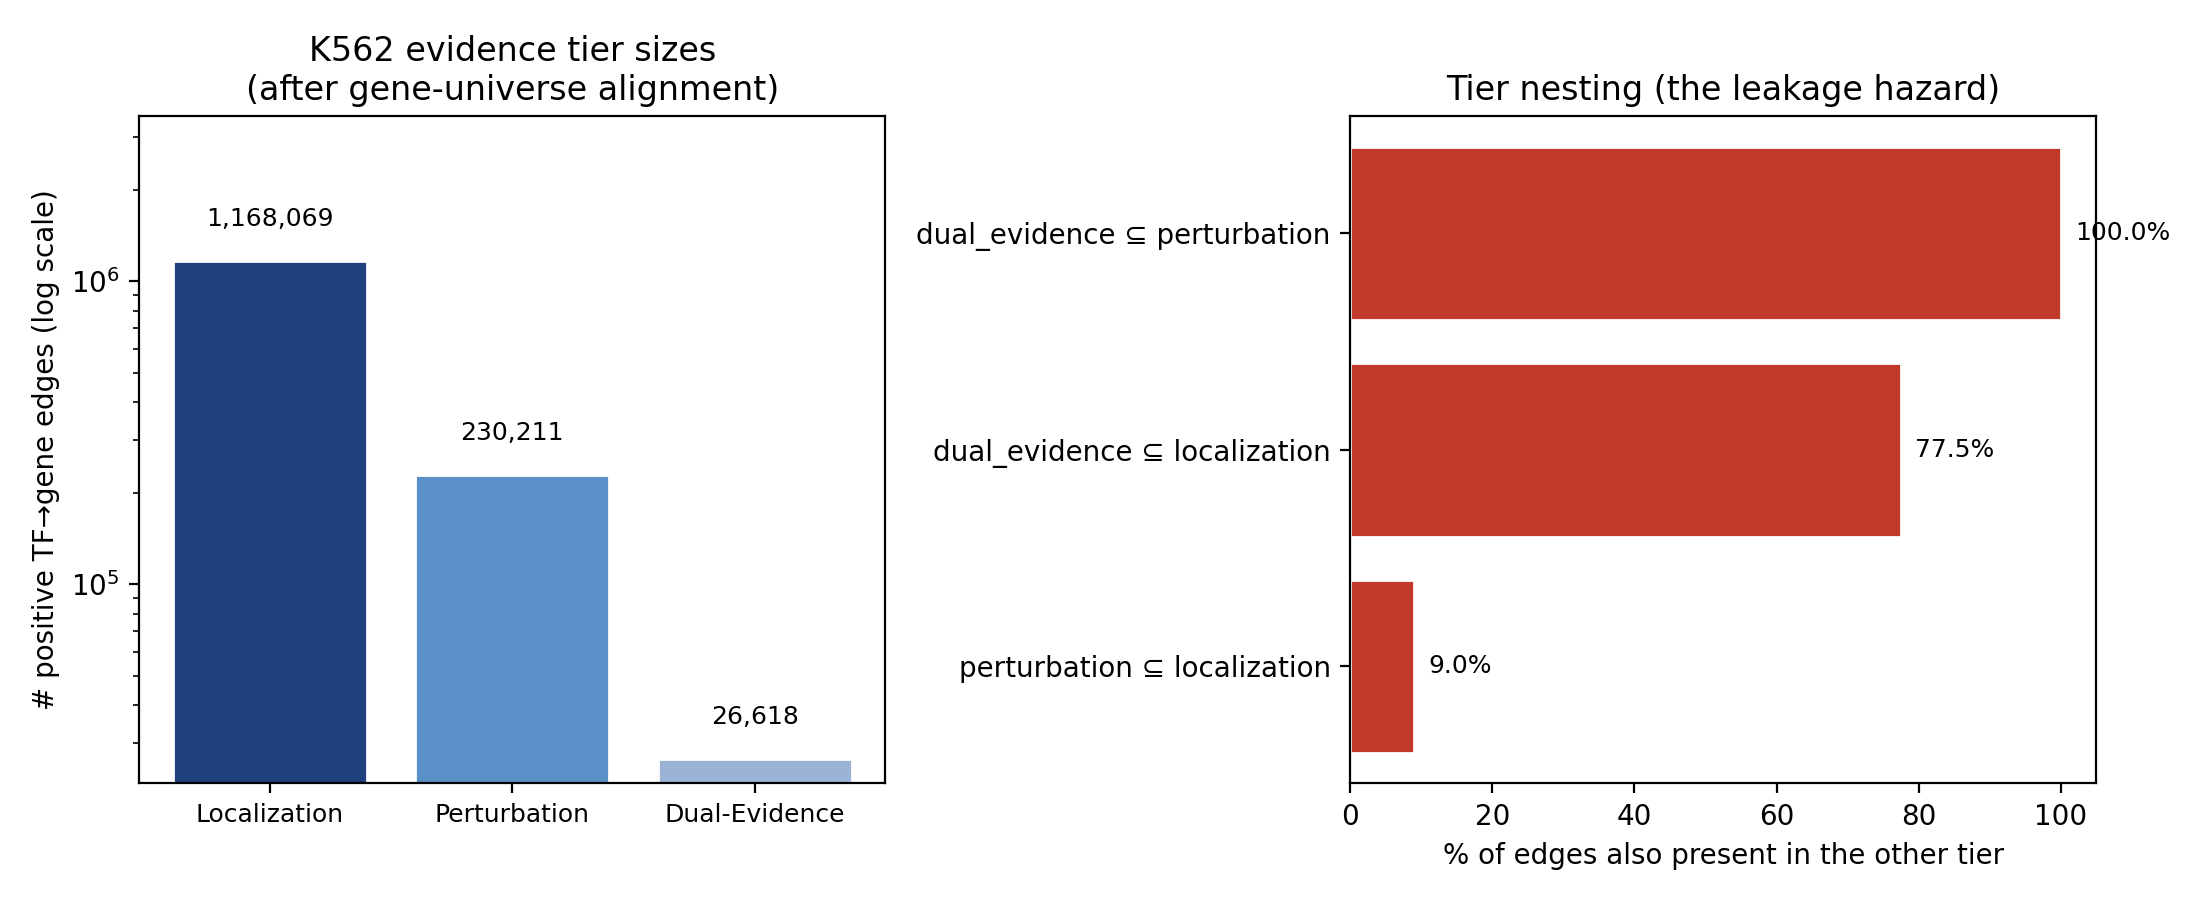
\includegraphics[width=\columnwidth]{figures/fig8_data_overview_nesting.png}
\caption{K562 evidence-tier sizes (left) and pairwise nesting fractions
(right). Perturbation is a largely disjoint, high-precision complement to
localization ($9.0\%$ overlap), while dual-evidence is almost entirely a
subset of both ($100\%$ of dual-evidence $\subseteq$ perturbation, $77.5\%$
$\subseteq$ localization).}
\label{fig:nesting}
\end{figure}

\subsection{A global, hierarchy-consistent splitting protocol}
\label{sec:split}
Because the tiers are nested rather than disjoint, splitting each tier
\emph{independently} into train/validation/test (as is standard practice when
tiers are assumed unrelated) does not, by itself, guarantee that a
(TF, gene) pair assigned to one tier's evaluation split is absent from another
tier's training split -- an independent random draw per tier can place the same
underlying edge into different splits for different tiers. Since this is exactly
the situation created by the nesting quantified in Section \ref{sec:nesting}, we
instead adopt a splitting protocol that assigns a single, global split label to
every unique (TF, gene) pair, once, across the \emph{union} of all evidence
tiers, and then defines each tier's own train/validation/test partition as the
intersection of that tier's edge set with the global assignment.

\begin{algorithm}[t]
\caption{Global hierarchy-consistent edge splitting}
\label{alg:split}
\begin{algorithmic}
\STATE {\bfseries Input:} tier edge sets $E_{\text{loc}}, E_{\text{pert}},
E_{\text{dual}}$; ratios $(r_{\text{tr}}, r_{\text{val}}, r_{\text{te}}) =
(0.70, 0.15, 0.15)$; seed
\STATE $U \leftarrow E_{\text{loc}} \cup E_{\text{pert}} \cup E_{\text{dual}}$
\hfill{\small\it pool unique pairs across all tiers}
\STATE Shuffle $U$ deterministically with \emph{seed}
\STATE Partition the shuffled $U$ into $(U_{\text{tr}}, U_{\text{val}},
U_{\text{te}})$ by $(r_{\text{tr}}, r_{\text{val}}, r_{\text{te}})$
\STATE $\pi(e) \leftarrow s$ for every $e \in U_s$, $s \in \{\text{tr}, \text{val}, \text{te}\}$
\FOR{each tier $t \in \{\text{loc}, \text{pert}, \text{dual}\}$}
\FOR{each split $s \in \{\text{tr}, \text{val}, \text{te}\}$}
\STATE $\text{split}_t(s) \leftarrow E_t \cap \pi^{-1}(s)$
\ENDFOR
\ENDFOR
\STATE {\bfseries Output:} per-tier splits $\{\text{split}_t(s)\}$
\end{algorithmic}
\end{algorithm}

Because $\pi$ assigns exactly one split label per unique pair, independent of
which tier(s) that pair happens to belong to, Algorithm \ref{alg:split}
satisfies a structural non-leakage property by construction:

\begin{proposition}[Cross-tier split consistency]
\label{prop:split}
Let $\pi$ be the global assignment produced by Algorithm \ref{alg:split}. For
any two tiers $t, t'$ and any edge $e \in E_t \cap E_{t'}$, $e$ is assigned to
the \emph{same} split under both tiers: $e \in \mathrm{split}_t(s)
\Leftrightarrow e \in \mathrm{split}_{t'}(s)$. Consequently, no edge can be a
training positive under one tier while simultaneously being a validation or
test positive under another tier.
\end{proposition}

Proposition \ref{prop:split} is what licenses the zero-shot evaluation
methodology in Section \ref{sec:curriculum}: any dual-evidence edge that falls
in $\pi^{-1}(\text{val}) \cup \pi^{-1}(\text{test})$ is guaranteed to not have
been a training positive under localization or perturbation either, however
deeply dual-evidence is nested inside them. We use 5 sampled negatives per
positive for training and 5 for evaluation, drawn from a pre-sampled pool of
1{,}000{,}000 random non-positive TF$\times$gene pairs; we verified in early
experiments that ranking negatives by chromatin accessibility (rather than
sampling them uniformly at random) inflates AUPR through an expression-level
artifact unrelated to genuine regulatory signal, and therefore use uniform
random negative sampling throughout.

\section{Model Architecture}
\label{sec:model}

\subsection{Design philosophy}
RNA and ATAC are not interchangeable evidence for the same underlying quantity;
they answer two different biological questions. Whether TF~$i$ can regulate
gene~$j$ depends on (a) whether $j$'s locus is \emph{accessible} -- an ATAC
property, and a \emph{precondition} rather than a graded signal -- and (b)
whether $i$ and $j$ are transcriptionally \emph{compatible}, e.g.\ co-expressed
across the same cell states -- an RNA property. MEvD-GRN reflects this
asymmetry structurally: RNA and ATAC are encoded and message-passed in two
separate towers that never mix until the very last step, the decoder, where
the ATAC representation acts as a multiplicative \emph{gate} on the RNA
representation rather than being concatenated or averaged with it.

\subsection{Modality encoders}
Each gene $g$ is represented by two small feature vectors, built once per cell
type from the single-cell data (Section \ref{sec:data}): an RNA feature
$x^{\text{rna}}_g \in \mathbb{R}^3$ (mean expression, variance, detection rate)
concatenated with a 50-dimensional co-expression signature $s_g$ obtained from
a truncated SVD of the standardized expression matrix such that $s_i \cdot s_j
\approx \mathrm{corr}(g_i, g_j)$ without ever materializing the dense
gene$\times$gene correlation matrix; and an ATAC feature $x^{\text{atac}}_g \in
\mathbb{R}^2$ (mean and variance of gene-activity score), with a scalar locus
openness feature used later, only at the decoder.

\begin{align}
h^{\text{rna}}_g &= \mathrm{LN}\!\big(W_2\, \mathrm{Dropout}(\mathrm{GELU}(\mathrm{LN}(W_1 x^{\text{rna}}_g)))\big) \\
h^{\text{atac}}_g &= \mathrm{LN}\!\big(\mathrm{GELU}(W_a x^{\text{atac}}_g)\big)
\end{align}

with $W_1 \in \mathbb{R}^{64\times3}$, $W_2 \in \mathbb{R}^{128\times64}$, $W_a
\in \mathbb{R}^{128\times2}$, mapping both modalities into a shared 128-d
space that is nonetheless kept in \emph{separate tensors} per modality.

\subsection{Dual relational GNN towers}
Two message-passing graphs, built once from structure only (never from labeled
positive edges, to avoid leaking label information into the node embeddings
themselves), are shared by both modality towers: a gene--gene co-expression
$k$NN graph ($k=20$, undirected) capturing co-regulation modules, and a
TF$\to$candidate-target graph connecting each TF to its top-500 accessible and
co-expressed targets (directionality is used only to construct the graph; the
graph is treated as bidirectional for message passing, and directionality is
reintroduced only at the decoder). Each tower is a 2-layer relational
GraphSAGE \cite{hamilton2017graphsage}: every layer runs one \texttt{SAGEConv}
per relation and sums the results before a shared LayerNorm + GELU + dropout,
so a node's updated representation mixes both co-expression neighbors and
regulatory-candidate neighbors at every layer:
\begin{equation}
h^{(\ell+1)} = \phi\Big(\textstyle\sum_{r \in \mathcal{R}} \mathrm{SAGE}_r^{(\ell)}\big(h^{(\ell)}\big)\Big)
\end{equation}
where $\mathcal{R} = \{\text{coexpr}, \text{TF-cand}\}$ and $\phi = \mathrm{Dropout}
\circ \mathrm{GELU} \circ \mathrm{LN}$, applied identically, but with
independent weights, to the RNA tower ($h^{\text{rna}}$) and the ATAC tower
($h^{\text{atac}}$).

\subsection{Role-aware decoder}
The decoder is where the two modalities finally interact, and it does so
asymmetrically by design: ATAC gates RNA, not the reverse.
\begin{align}
a_j &= \sigma\big(W_{\text{gate}}\, h^{\text{atac}}_j\big) \\
z_j &= h^{\text{rna}}_j \odot a_j \\
\text{raw} &= (h^{\text{rna}}_i)^{\!\top} W\, z_j \\
\text{logit} &= \text{raw} + w_c \cdot \mathrm{coexpr}(i,j) + w_o \cdot \mathrm{open}_j + b
\end{align}
Here $a_j \in [0,1]^{128}$ is a per-dimension \emph{accessibility gate}
derived from the target's ATAC embedding; $z_j$ is the target's resulting
``regulatable'' RNA state; \text{raw} is an asymmetric bilinear TF$\to$target
compatibility score; and $\mathrm{coexpr}(i,j) = s_i \cdot s_j$ is the
co-expression-signature dot product, while $\mathrm{open}_j$ is the
locus-openness scalar from Section \ref{sec:data}. Both additive terms let
the decoder fall back on direct co-expression and raw accessibility evidence
even when the learned bilinear term is uncertain. The model outputs logits;
sigmoid is applied only at the loss/eval boundary.

\subsection{Parameter budget}
Table \ref{tab:params} breaks down the 306{,}691 trainable parameters by
module. For reference, this is roughly \textbf{13$\times$ smaller} than a
single scMultiomeGRN model (4{,}077{,}914 parameters; Section
\ref{sec:baselines}). Figure \ref{fig:arch} shows the full architecture.

\begin{table}[t]
\caption{MEvD-GRN parameter count by module.}
\label{tab:params}
\vskip 0.1in
\begin{center}
\begin{small}
\begin{tabular}{lr}
\toprule
Module & Parameters \\
\midrule
RNA encoder (MLP, $3\to64\to128$) & 8{,}960 \\
ATAC encoder (linear, $2\to128$) & 640 \\
GNN$_{\text{RNA}}$ tower (2-layer rel.\ SAGE) & 132{,}096 \\
GNN$_{\text{ATAC}}$ tower (2-layer rel.\ SAGE) & 132{,}096 \\
Role-aware decoder & 32{,}899 \\
\midrule
\textbf{Total} & \textbf{306{,}691} \\
\bottomrule
\end{tabular}
\end{small}
\end{center}
\end{table}

\begin{figure}[t]
\centering
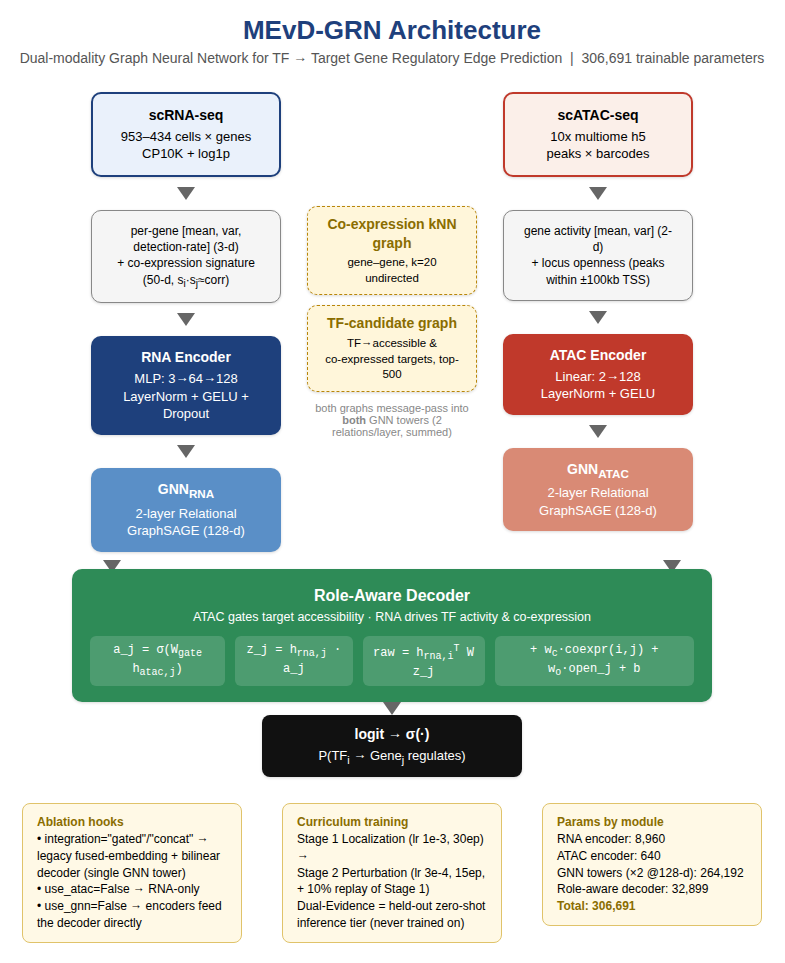
\includegraphics[width=\columnwidth]{figures/architecture_diagram.png}
\caption{MEvD-GRN architecture. RNA and ATAC signals are encoded and
message-passed in separate towers over two shared structural graphs
(co-expression $k$NN and TF-candidate), and combine only at the role-aware
decoder, where the ATAC embedding gates the RNA embedding before an asymmetric
bilinear compatibility score is computed.}
\label{fig:arch}
\end{figure}

\subsection{Architectural ablation hooks}
Three flags let us isolate the contribution of each design choice
experimentally (Section \ref{sec:ablation}): \texttt{integration=gated/concat}
replaces the role-aware decoder with a single fused embedding and a classical
asymmetric bilinear decoder; \texttt{use\_atac=False} zeroes the ATAC branch
entirely (RNA-only); and \texttt{use\_gnn=False} feeds encoder outputs directly
to the decoder, removing message passing altogether.

\section{Training Strategy}
\label{sec:curriculum}

\subsection{A two-stage evidence-tier curriculum}
\label{sec:two-stage}
MEvD-GRN is trained sequentially: Stage 1 on the localization tier (30 epochs,
learning rate $10^{-3}$), then Stage 2 on the perturbation tier (15 epochs,
learning rate $3{\times}10^{-4}$), both with the full network unfrozen. We
deliberately \emph{exclude} the dual-evidence tier from training altogether and
reserve it as a zero-shot generalization benchmark, evaluated only at
inference time after Stage 2. This is not merely a convenient simplification;
it is motivated directly by the nesting structure quantified in Section
\ref{sec:nesting}. Because dual-evidence is $100\%$ contained in perturbation
and $77.5\%$ contained in localization at K562, a model that is fine-tuned
directly on dual-evidence edges would, for the large majority of those edges,
be fitting labels for (TF, gene) pairs whose regulatory relationship it has
already substantially been exposed to in an upstream tier -- so a good score
on a held-out \emph{split} of dual-evidence edges would conflate genuine
generalization to the highest-confidence tier with memorization of a
near-duplicate of what was already trained on. Evaluating a model that has
\emph{never seen a single dual-evidence gradient update} sidesteps this
ambiguity entirely: by Proposition \ref{prop:split}, every dual-evidence edge
used at evaluation time is guaranteed to not have been a positive example under
\emph{any} tier's training split, making the resulting score an unambiguous
measurement of transfer to the highest-confidence evidence tier rather than a
measurement of fine-tuning capacity. We treat this zero-shot dual-evidence
score as the paper's headline generalization metric (Section
\ref{sec:results}).

Evaluation follows a matching convention (\textsc{EvalEdgesForTier}): tiers
that were trained on (localization, perturbation) are scored on their
\emph{test} split only, exactly as in standard practice; the held-out
dual-evidence tier, having no training split to speak of, is scored on its
\emph{validation + test} splits combined, since both are equally unseen and
combining them yields a larger, less noisy estimate.

\subsection{Hard-negative mining}
For each training stage, half of the sampled negative pairs are drawn
uniformly at random from the global negative pool (Section \ref{sec:data});
the other half are \emph{hard negatives} -- pairs that are positive in an
easier tier of the hierarchy but not in the current training tier. This
forces the decoder to distinguish ``binds but does not (yet, functionally)
regulate'' from ``binds and regulates,'' rather than learning a shortcut
that conflates the two notions.

\subsection{Memory replay: mechanism and an honest quantitative result}
\label{sec:replay}
During Stage 2, a small fraction (\texttt{replay\_weight}=$0.1$, i.e.\ $10\%$
of the current batch size) of Stage 1's localization positives are re-injected
into every batch at reduced loss weight ($0.1$), in the spirit of experience
replay \cite{rolnick2019replay}. We report the effect of this mechanism
honestly rather than presenting it as a solved problem. Table
\ref{tab:forgetting} shows localization AUROC measured \emph{after} Stage 2
completes, under three conditions:

\begin{table}[t]
\caption{Catastrophic forgetting of the localization tier after Stage 2, and
how much of it different mitigations recover. AUROC $<0.5$ indicates the
model's ranking is worse than random on the forgotten tier.}
\label{tab:forgetting}
\vskip 0.1in
\begin{center}
\begin{small}
\begin{tabular}{lc}
\toprule
Configuration & Localization AUROC \\
\midrule
No replay (2-stage) & 0.290 \\
Replay, 2-stage (\textbf{shipped default}) & 0.326 \\
Replay, full 3-stage + consolidation & 0.736 \\
\bottomrule
\end{tabular}
\end{small}
\end{center}
\end{table}

Replay alone, within the two-stage curriculum actually used by the shipped
model, provides only a modest recovery ($0.290 \to 0.326$) and does not resolve
the underlying problem: post-Stage-2 localization AUROC remains \emph{below
random} ($<0.5$). The much larger recovery ($0.736$) is achieved only by a
qualitatively different recipe -- a full three-stage curriculum that adds a
frozen-encoder consolidation pass with replay over all tiers -- which we study
as an ablation (\texttt{with\_replay}, Section \ref{sec:ablation}) rather than
adopt as the shipped default, precisely because isolating \emph{why} replay
alone under-performs is itself an informative result (Section
\ref{sec:discussion}).

\subsection{Optimization details}
We use AdamW (weight decay $10^{-4}$), gradient-norm clipping at $1.0$, batch
size $8{,}192$, and cosine learning-rate decay within each stage. The loss is a
class-balanced weighted binary cross-entropy with $\text{pos\_weight} =
n_{\text{neg}}/n_{\text{pos}}$ recomputed per stage. We use early stopping on
validation AUPR with a patience of 10 checks, evaluating every 5 epochs.
End-to-end training of the shipped 2-stage model takes \textbf{16.6 minutes} on
a single consumer GPU (RTX 4060).

\begin{figure}[t]
\centering
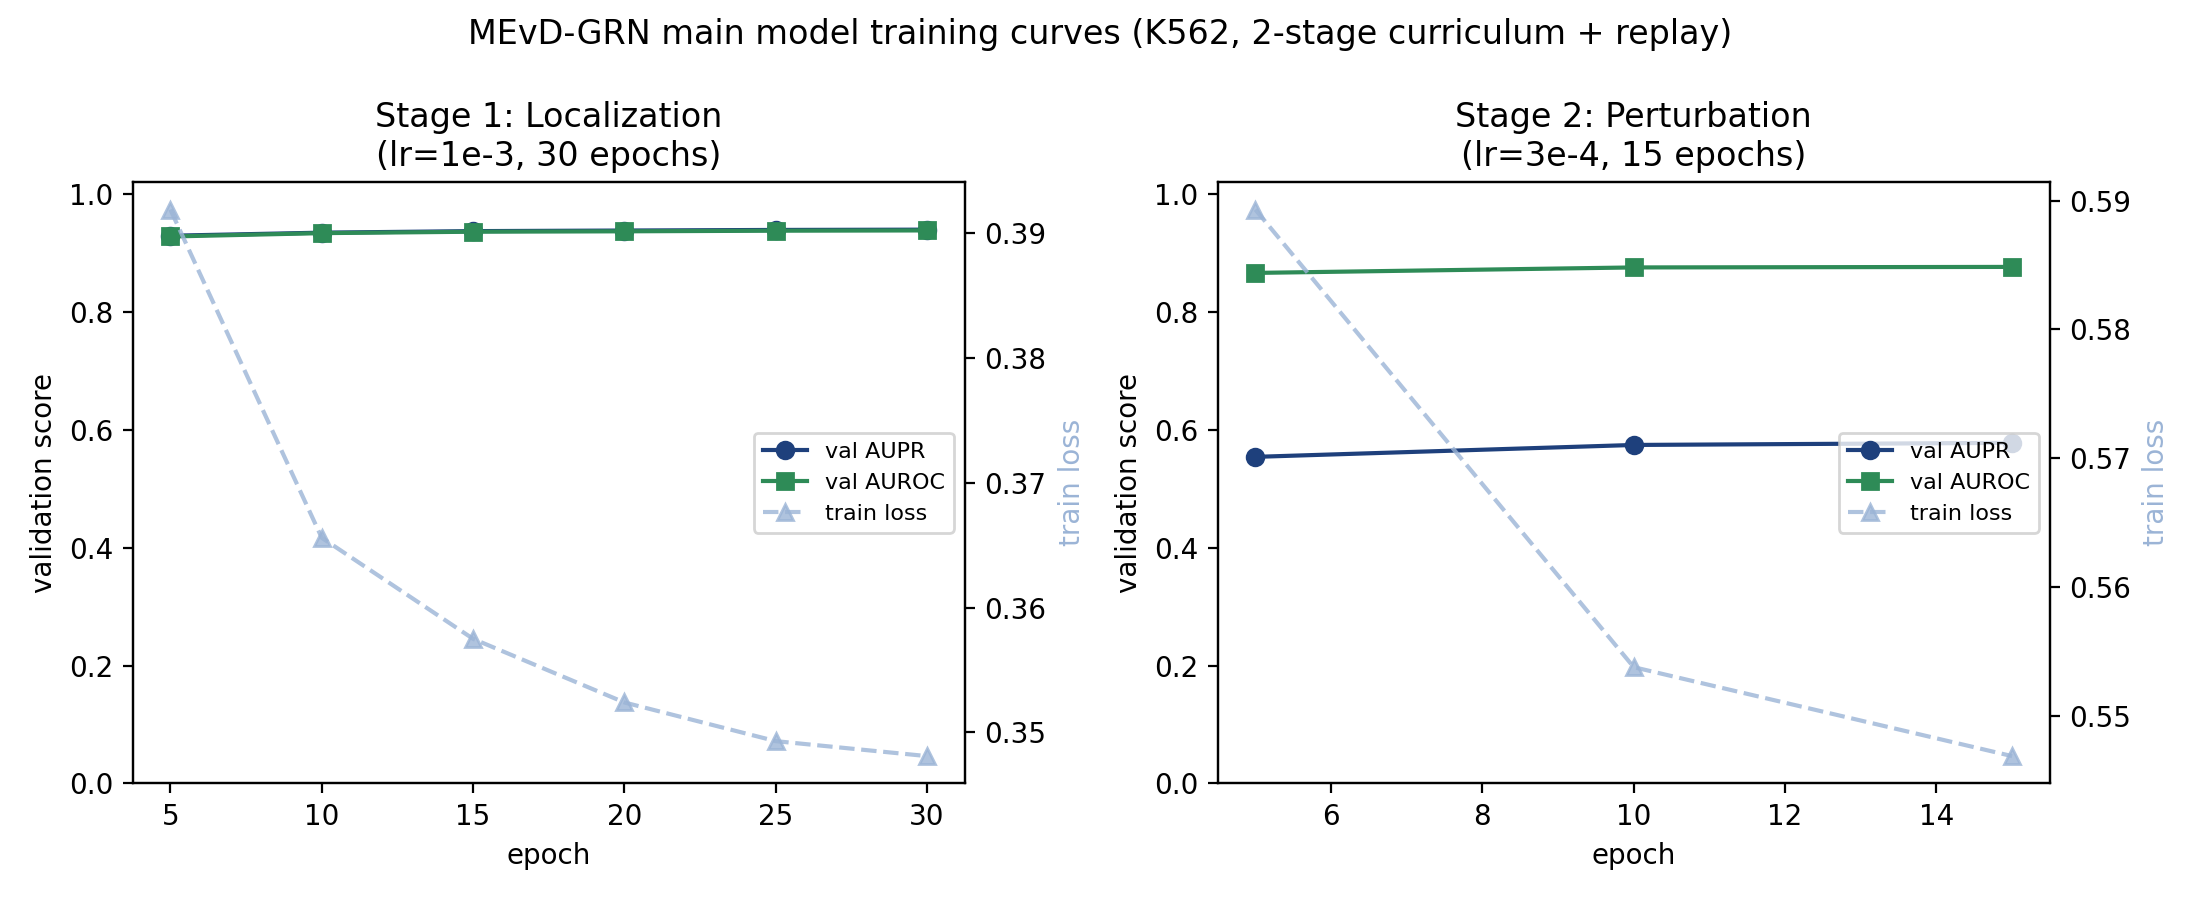
\includegraphics[width=\columnwidth]{figures/fig7_training_curves.png}
\caption{K562 training curves for the shipped 2-stage model. Stage 1 converges
smoothly to validation AUPR/AUROC $\approx 0.94$ on localization. Stage 2's own
validation curve (perturbation, AUROC $0.876$) looks healthy in isolation --
the forgetting reported in Table \ref{tab:forgetting} is invisible from Stage
2's own curve and appears only when Stage 1's tier is re-evaluated afterward.}
\label{fig:curves}
\end{figure}

\section{Evaluation Protocol}
\label{sec:eval}

We report four metrics, computed per evidence tier: \textbf{AUPR}, the area
under the precision-recall curve, our primary metric because it is far more
sensitive than AUROC to the severe class imbalance inherent to link prediction
over a candidate space where true edges are $\ll 1\%$ of all pairs;
\textbf{AUROC}, the area under the ROC curve, retained as a secondary metric
because it exposes below-random ranking that AUPR alone can mask (as in Table
\ref{tab:forgetting}); \textbf{Early Precision (EP)}, the precision restricted
to the top-$k$ scored candidate pairs with $k$ set to the number of true
positives, which measures how useful the very top of a ranked candidate list
is in practice; and \textbf{EPR}, EP normalized by the random-guessing base
rate over the \emph{full} bipartite candidate space
($225\times22{,}942=5{,}161{,}950$ pairs, following the BEELINE enrichment
convention). Because the candidate space is enormous relative to the positive
set, EPR values of $10^1$--$10^3$ are expected even when the corresponding AUPR
looks numerically modest.

\section{Baselines}
\label{sec:baselines}

We compare against four baselines, all evaluated on the \emph{identical}
splits and evaluation convention as MEvD-GRN (Algorithm \ref{alg:split},
Section \ref{sec:two-stage}), for a fully apples-to-apples comparison.
\textbf{GRNBoost2} \cite{moerman2019grnboost2} is the field-standard
tree-ensemble co-expression method (RNA-only, non-parametric).
\textbf{RegDiffusion} \cite{zhu2024regdiffusion} is a diffusion-based GRN
inference model (RNA-only); we restrict its input gene set to highly-variable
genes and TFs to avoid zero-variance instabilities introduced by its internal
normalization. \textbf{GMF-GAE} is a graph-autoencoder baseline over the
co-expression $k$NN graph, standing in for the GMFGRN family
\cite{li2024gmfgrn} (RNA-only). \textbf{scMultiomeGRN}
\cite{xu2025scmultiomegrn} is the strongest baseline: a supervised multi-omic
GNN with cross-modal attention, at 4{,}077{,}914 parameters \emph{per trained
tier} (it fits a dedicated model per tier rather than sharing weights across a
curriculum, so it never experiences catastrophic forgetting by construction).
Its original formulation targets TF$\leftrightarrow$TF interactions; we adapt
it to our TF$\to$all-genes benchmark, decoding edges sparsely so the full
$|\mathcal{V}_{\text{TF}}|\times|\mathcal{V}_{\text{gene}}|$ score matrix is
never materialized. We train it for 100 epochs per tier (an exploratory
budget; its published default is 2{,}000 epochs -- see Section
\ref{sec:limitations}).

\section{Results}
\label{sec:results}

\subsection{Main results}
Table \ref{tab:main} reports MEvD-GRN's performance on all three evidence
tiers. The headline result is the dual-evidence row: evaluated in a strict
zero-shot setting (Section \ref{sec:two-stage}), the model reaches AUPR
$0.558$ / AUROC $0.838$ on a tier it never received a single gradient update
from -- evidence of genuine transfer rather than memorization, a claim made
rigorous by Proposition \ref{prop:split}. The localization row, however,
carries the caveat quantified in Section \ref{sec:replay}: AUROC $0.326$ is
below random, the direct, visible cost of catastrophic forgetting.

\begin{table}[t]
\caption{MEvD-GRN main results on K562. Localization/perturbation are scored
on their test split (trained tiers); dual-evidence is scored on
validation+test, zero-shot (never trained on).}
\label{tab:main}
\vskip 0.1in
\begin{center}
\begin{small}
\begin{tabular}{lcccc}
\toprule
Tier & AUPR & AUROC & EP & EPR \\
\midrule
Localization$^\dagger$ & 0.420 & 0.326 & 0.425 & 12.5 \\
Perturbation & 0.575 & 0.876 & 0.536 & 80.2 \\
Dual-evidence$^\ddagger$ & \textbf{0.558} & \textbf{0.838} & 0.419 & 272.5 \\
\bottomrule
\end{tabular}
\end{small}
\end{center}
\vskip -0.05in
{\footnotesize $^\dagger$affected by catastrophic forgetting, Section
\ref{sec:replay}. $^\ddagger$zero-shot, never trained on.}
\end{table}

\begin{figure}[t]
\centering
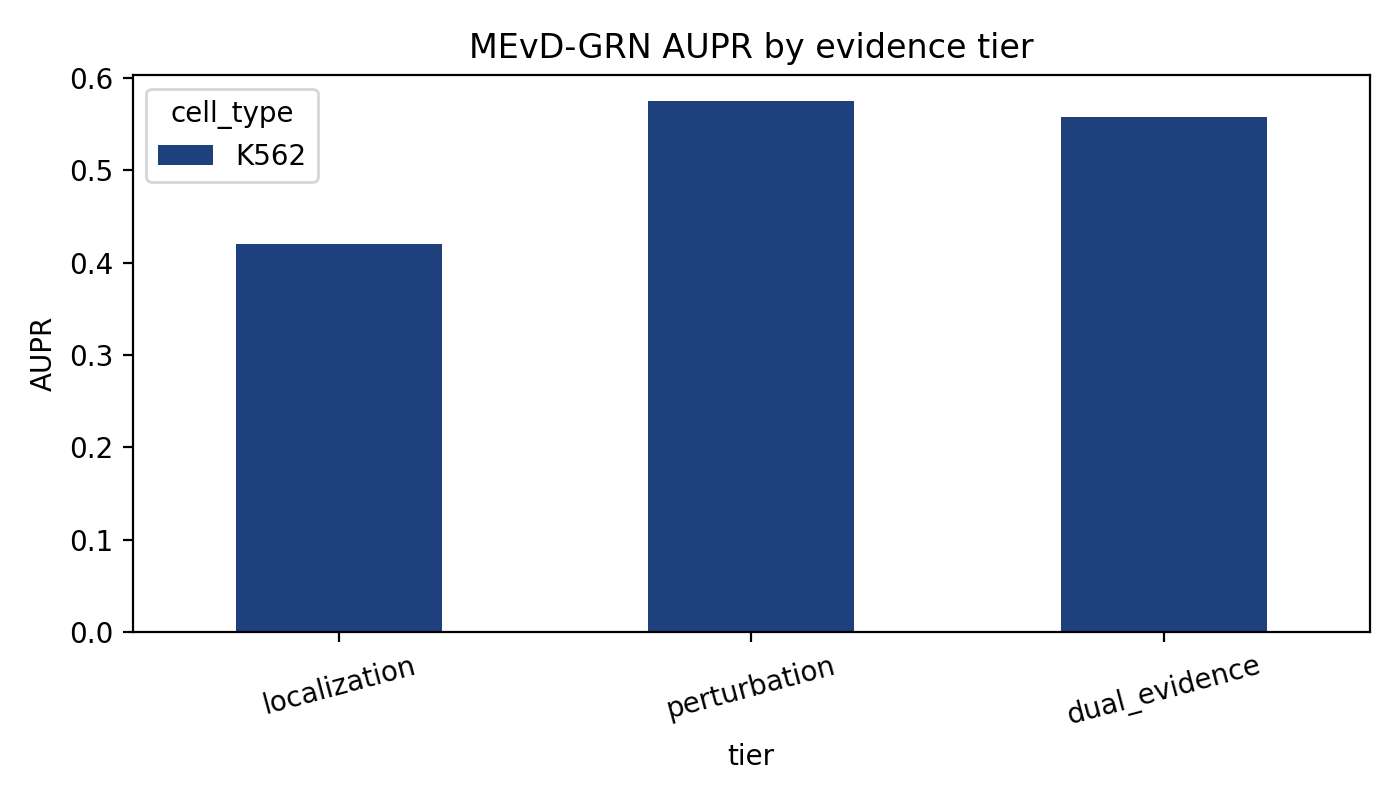
\includegraphics[width=\columnwidth]{figures/fig1_mevdgrn_per_tier.png}
\caption{MEvD-GRN AUPR by evidence tier on K562.}
\label{fig:per-tier}
\end{figure}

\begin{figure}[t]
\centering
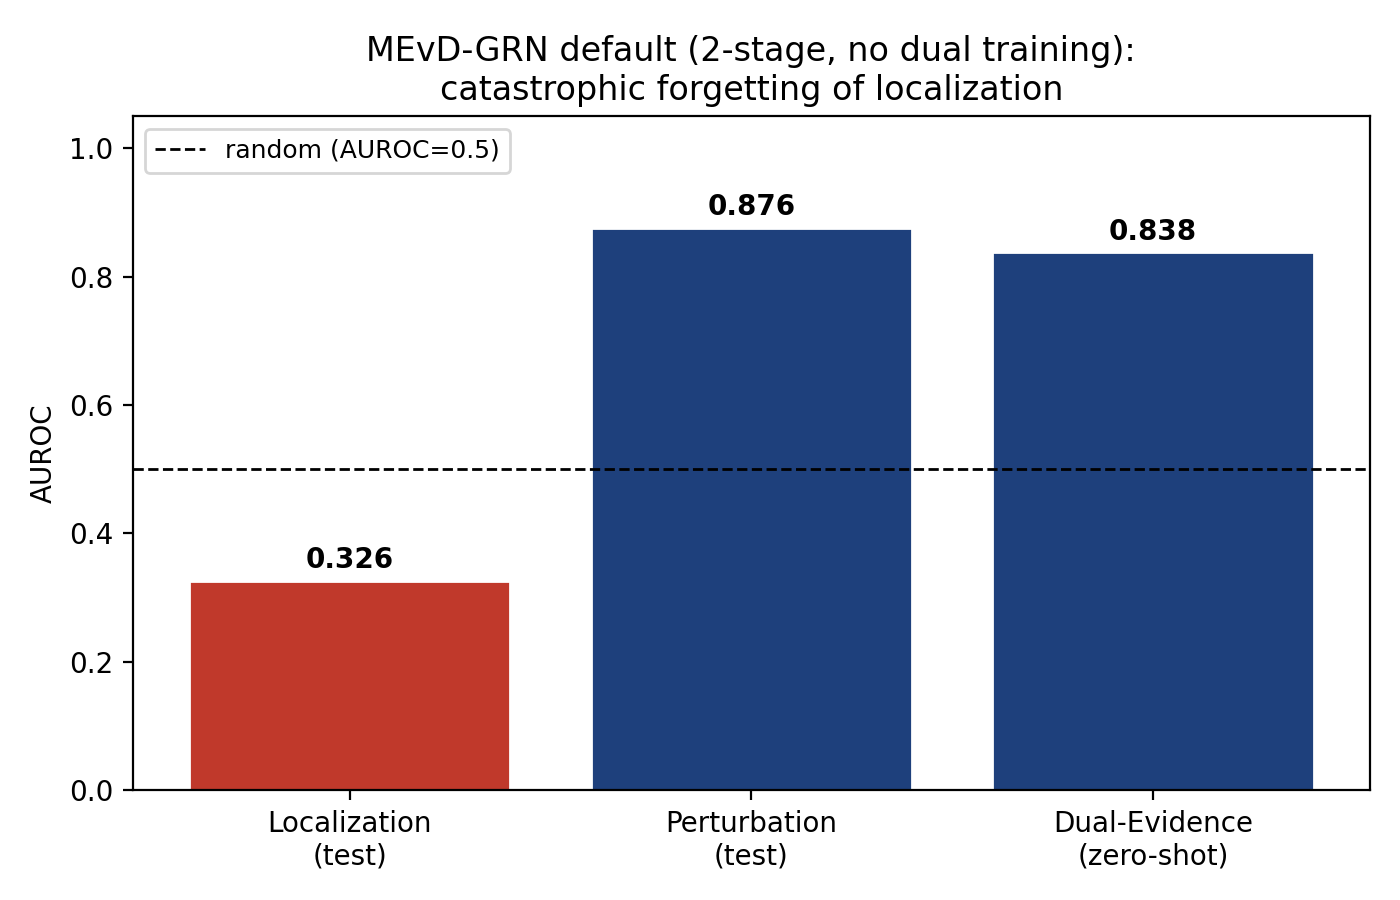
\includegraphics[width=\columnwidth]{figures/fig5_catastrophic_forgetting_auroc.png}
\caption{Localization AUROC over the curriculum: Stage 1 reaches
$\approx0.94$, then collapses to $0.326$ after Stage 2 -- below the $0.5$
random-ranking line (dashed).}
\label{fig:forgetting}
\end{figure}

\subsection{Comparison against baselines}
Table \ref{tab:baselines} compares AUPR across all five methods on all three
tiers. scMultiomeGRN dominates localization ($0.831$ AUPR), which is expected:
it fits a dedicated model per tier with no sequential fine-tuning and hence no
forgetting, at roughly $13\times$ the parameter count of a single MEvD-GRN
model. MEvD-GRN wins clearly on perturbation and, more importantly, on
dual-evidence \emph{under true zero-shot transfer} -- despite never training
on that tier and using a fraction of the parameters. The RNA-only classical and
diffusion baselines (GRNBoost2, RegDiffusion, GMF-GAE) trail on every tier,
consistent with none of them exploiting chromatin accessibility or the
evidence-tier structure.

\begin{table}[t]
\caption{AUPR comparison across methods and tiers, K562. Dual-evidence AUPR
for MEvD-GRN is a zero-shot score; all other entries are in-distribution
(trained/fit on that tier).}
\label{tab:baselines}
\vskip 0.1in
\begin{center}
\begin{small}
\begin{tabular}{lccc}
\toprule
Method & Loc. & Pert. & Dual \\
\midrule
\textbf{MEvD-GRN} (ours) & 0.420 & \textbf{0.575} & \textbf{0.558} \\
scMultiomeGRN & \textbf{0.831} & 0.423 & 0.384 \\
GRNBoost2 & 0.535 & 0.206 & 0.173 \\
RegDiffusion & 0.546 & 0.185 & 0.165 \\
GMF-GAE & 0.526 & 0.218 & 0.160 \\
\bottomrule
\end{tabular}
\end{small}
\end{center}
\end{table}

\begin{figure}[t]
\centering
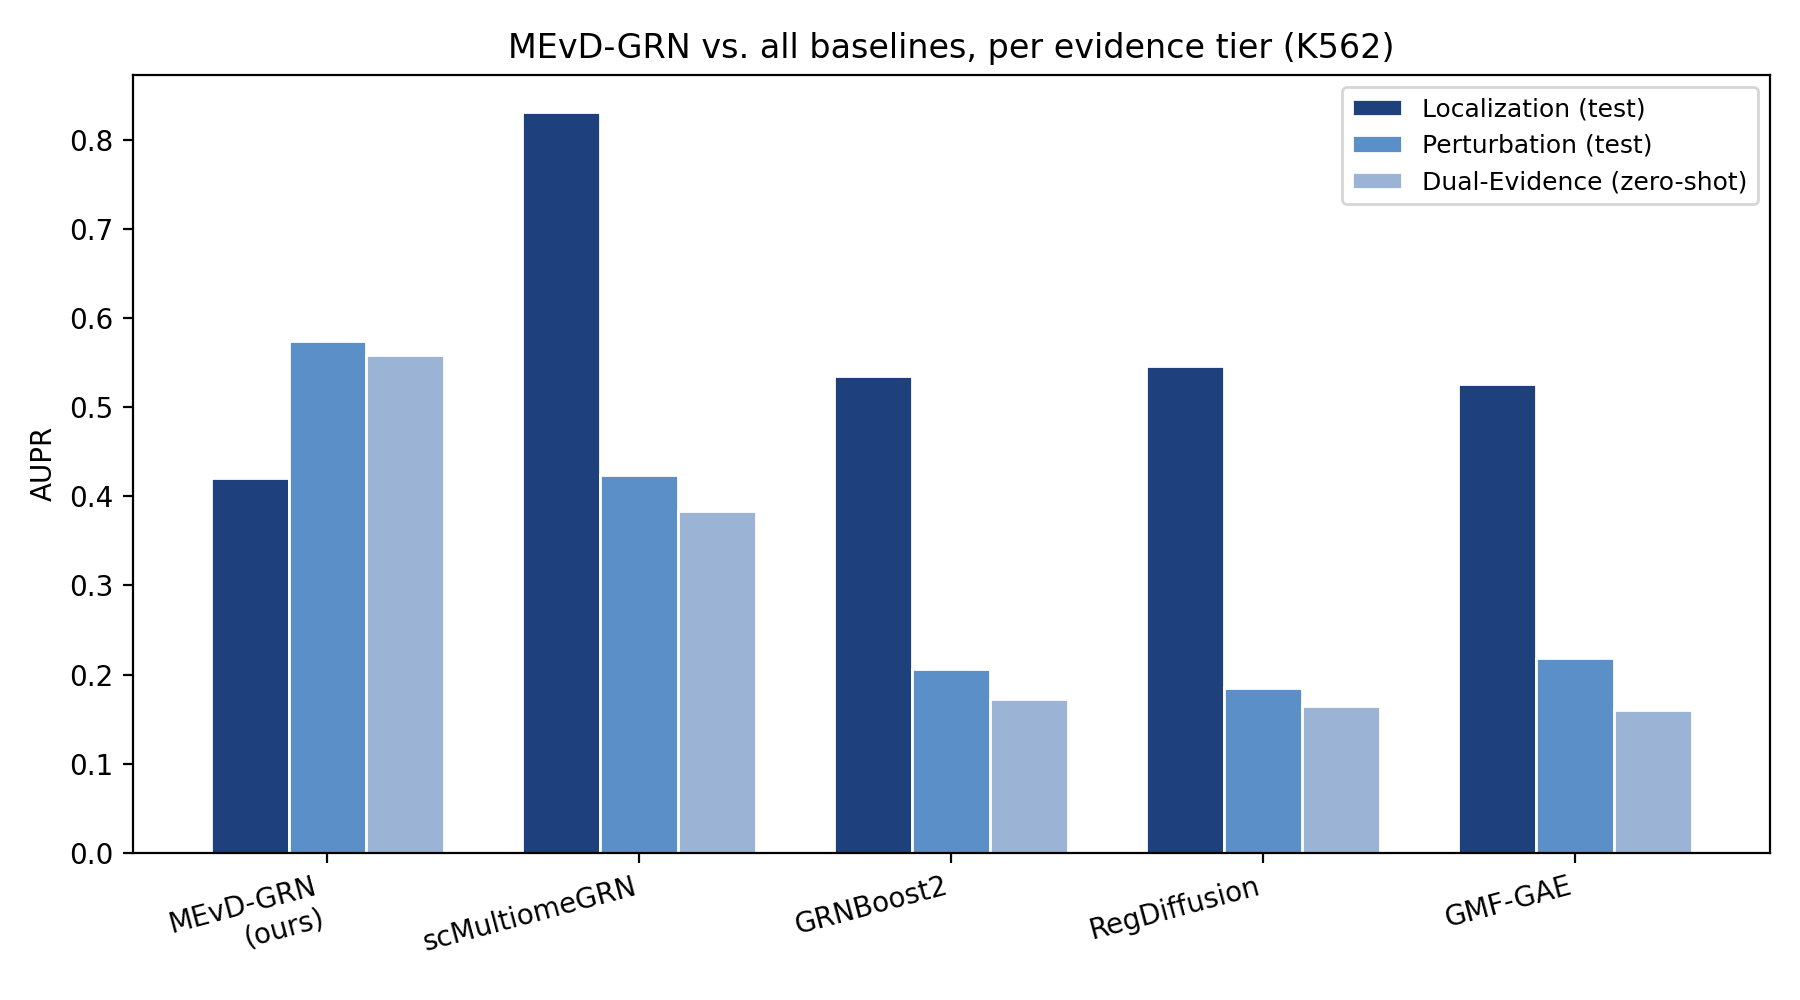
\includegraphics[width=\columnwidth]{figures/fig4_full_baseline_comparison.png}
\caption{Full per-tier AUPR comparison across all five methods.}
\label{fig:full-baselines}
\end{figure}

\subsection{Head-to-head against scMultiomeGRN under alternative curricula}
\label{sec:head2head}
Because scMultiomeGRN is the only baseline that is itself a supervised
multi-omic GNN, we examine it more closely, alongside two \emph{alternative}
MEvD-GRN training schedules already characterized by the ablation study
(Section \ref{sec:ablation}): \texttt{all\_at\_once} (localization and
perturbation trained jointly, no sequencing at all) and \texttt{with\_replay}
(the full three-stage curriculum with consolidation from Table
\ref{tab:forgetting}). Table \ref{tab:head2head} shows that no single
\emph{already-tested} MEvD-GRN configuration wins all three tiers outright,
but the choice of curriculum entirely determines which tiers are won: the
shipped default trades localization for a dual-evidence win, while
\texttt{with\_replay} very nearly ties scMultiomeGRN on both localization and
perturbation while beating it by $2.4\times$ on dual-evidence -- using
roughly $27\times$ fewer parameters than the three dedicated per-tier
scMultiomeGRN models such a sweep would otherwise require.

\begin{table*}[t]
\caption{Head-to-head vs.\ scMultiomeGRN across curriculum choices (K562, AUPR / AUROC). scMultiomeGRN uses a dedicated
4.08M-parameter model per tier; all three MEvD-GRN rows use the \emph{same} single 306{,}691-parameter model, only the
training schedule differs.}
\label{tab:head2head}
\vskip 0.1in
\begin{center}
\begin{small}
\begin{tabular}{lccc}
\toprule
Method (parameters) & Localization & Perturbation & Dual-evidence \\
\midrule
scMultiomeGRN (4.08M $\times$ up to 3 dedicated models) & \textbf{0.831} / \textbf{0.865} & 0.423 / 0.828 & 0.384 / 0.825 \\
MEvD-GRN --- shipped default, 2-stage (306{,}691 params) & 0.420 / 0.326 & \textbf{0.575} / \textbf{0.876} & 0.558 / 0.838 \\
MEvD-GRN --- \texttt{all\_at\_once} (same params) & \textbf{0.937} / \textbf{0.928} & 0.348 / 0.739 & \textbf{0.788} / 0.943 \\
MEvD-GRN --- \texttt{with\_replay} (same params) & 0.765 / 0.736 & 0.411 / 0.702 & \textbf{0.940} / \textbf{0.990} \\
\bottomrule
\end{tabular}
\end{small}
\end{center}
\end{table*}

\begin{figure}[t]
\centering
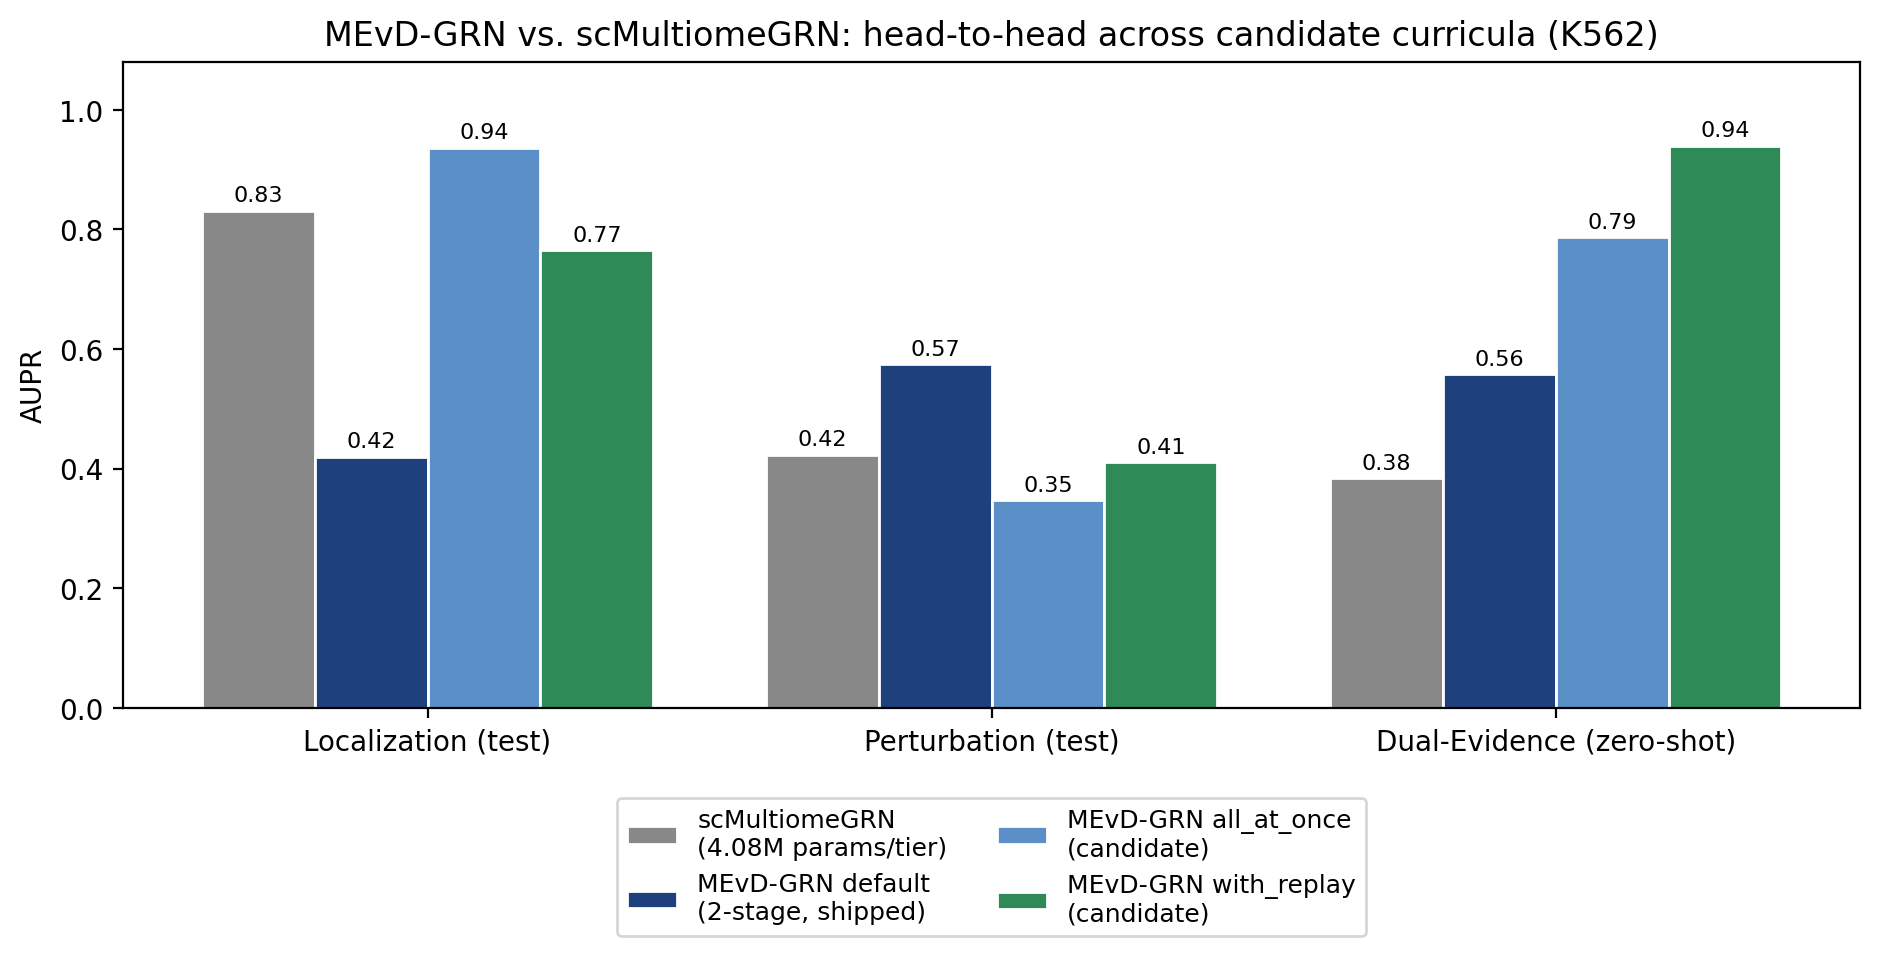
\includegraphics[width=\columnwidth]{figures/fig9_mevdgrn_vs_scmultiomegrn.png}
\caption{MEvD-GRN (three curricula) vs.\ scMultiomeGRN, AUPR by tier.}
\label{fig:head2head}
\end{figure}

\section{Ablation Study}
\label{sec:ablation}

We run 10 configurations under the identical splitting and evaluation protocol
(Section \ref{sec:eval}) to isolate the contribution of the curriculum, the
GNN backbone, the fusion strategy, and each modality. Table \ref{tab:ablation}
reports AUPR by tier for every configuration; AUROC/EP/EPR for all
configurations are given in Appendix \ref{app:full-ablation}.

\begin{table*}[t]
\caption{Ablation study, K562 (AUPR by tier). \texttt{full\_curriculum} is the shipped 2-stage default, reproduced here
as the reference row. \texttt{dual\_only} and \texttt{with\_replay} are explicit exceptions that do train on
dual-evidence, included to bound the comparison.}
\label{tab:ablation}
\vskip 0.1in
\begin{center}
\begin{small}
\begin{tabular}{llccc}
\toprule
Configuration & Trained on & Localization & Perturbation & Dual-evidence \\
\midrule
\texttt{full\_curriculum} (reference) & loc $\to$ pert, sequential & 0.410 & 0.569 & 0.546 \\
\texttt{loc\_only} & localization only & 0.940 & 0.187 & 0.663 \\
\texttt{pert\_only} & perturbation only & 0.407 & 0.496 & 0.485 \\
\texttt{dual\_only}$^*$ & dual-evidence only & 0.779 & 0.197 & 0.479 \\
\texttt{all\_at\_once} & loc + pert, simultaneous & \textbf{0.937} & 0.348 & \textbf{0.788} \\
\texttt{rna\_only} & loc $\to$ pert, ATAC zeroed & 0.414 & 0.540 & 0.543 \\
\texttt{gated\_fusion} & loc $\to$ pert, legacy fusion & 0.419 & 0.588 & 0.546 \\
\texttt{concat\_fusion} & loc $\to$ pert, plain concat & 0.421 & \textbf{0.595} & 0.555 \\
\texttt{no\_gnn} & loc $\to$ pert, no message passing & 0.498 & 0.341 & 0.241 \\
\texttt{with\_replay}$^*$ & full 3-stage + replay & 0.765 & 0.411 & \textbf{0.940} \\
\bottomrule
\end{tabular}
\end{small}
\end{center}
\vskip 0.02in
{\footnotesize $^*$deliberately trains on dual-evidence and is excluded from the zero-shot claim of Section \ref{sec:head2head}; included here for completeness.}
\end{table*}

\begin{figure}[t]
\centering
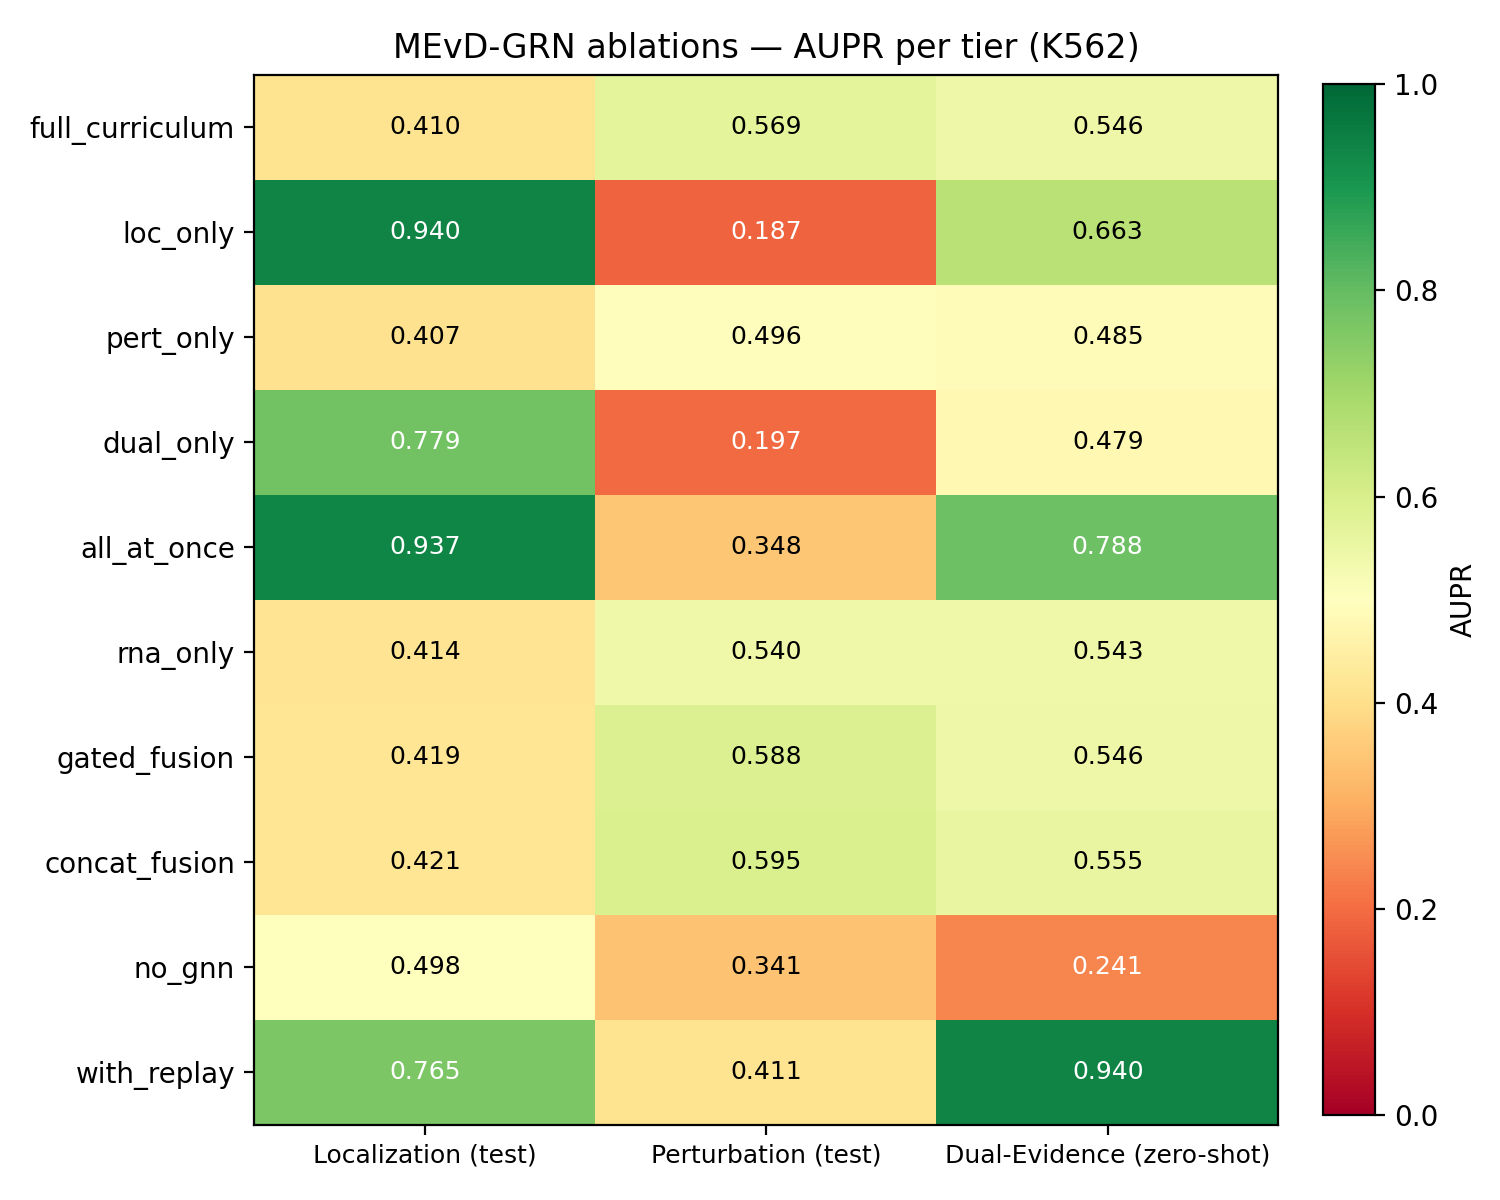
\includegraphics[width=\columnwidth]{figures/fig6_ablation_heatmap.png}
\caption{Ablation heatmap: AUPR by configuration $\times$ tier.}
\label{fig:ablation-heatmap}
\end{figure}

\subsection{Discussion of ablation findings}
\label{sec:discussion}

\textbf{Sequential ordering is not, by itself, beneficial once forgetting is
accounted for.} Comparing \texttt{full\_curriculum} against
\texttt{all\_at\_once} isolates the effect of \emph{sequencing} alone
(both train on the same two tiers, localization and perturbation; the only
difference is joint vs.\ sequential optimization): \texttt{all\_at\_once}
dominates on dual-evidence zero-shot generalization ($0.788$ vs.\ $0.546$
AUPR) and on localization ($0.937$ vs.\ $0.410$), while trading off a smaller
amount of perturbation performance ($0.348$ vs.\ $0.569$). This shows that the
sequential curriculum's advantage, if any, is more than offset by the
forgetting it introduces (Section \ref{sec:replay}) in the present
configuration -- a genuinely negative result for naive sequential ordering
that we report because it directly qualifies the curriculum-learning
hypothesis motivating this work.

\textbf{Replay with a consolidation pass recovers most of the deficit.}
\texttt{with\_replay}, which adds a third, frozen-encoder consolidation stage
with replay over all tiers on top of the sequential curriculum, achieves the
best dual-evidence score of any configuration ($0.940$ AUPR) and substantially
recovers localization ($0.765$, vs.\ $0.410$ for the plain sequential
curriculum), at some cost to perturbation ($0.411$ vs.\ $0.569$). Combined
with the \texttt{all\_at\_once} result, this suggests two independently
viable routes to a stronger default recipe than the currently shipped one
(Section \ref{sec:limitations}).

\textbf{The GNN backbone is the single highest-value architectural
component.} \texttt{no\_gnn} is the worst configuration on every tier
(localization $0.498$, perturbation $0.341$, dual $0.241$), confirming that
relational message passing over the co-expression and TF-candidate graphs
contributes substantially more than any other architectural choice we
ablate.

\textbf{Fusion style is a second-order effect at the point-metric level.}
Role-aware, gated, and concatenation fusion land within $\approx 0.02$--$0.03$
AUPR of one another under the shipped curriculum (Table
\ref{tab:ablation}, rows \texttt{full\_curriculum}/\texttt{gated\_fusion}/
\texttt{concat\_fusion}); the role-aware decoder's advantage is currently more
interpretive/biologically-motivated (Section \ref{sec:model}) than a large
raw-metric win, and we flag this honestly as an open question rather than
overstate it.

\textbf{ATAC's marginal contribution is currently small.}
\texttt{rna\_only} (ATAC branch zeroed) performs almost identically to the
full model ($0.414$/$0.540$/$0.543$ vs.\ $0.410$/$0.569$/$0.546$), suggesting
that under the current coarse, gene-level (mean/variance) ATAC featurization,
chromatin accessibility is not yet contributing information that the RNA
co-expression signature does not already capture. We view this as an artifact
of the featurization rather than a fundamental property of the data, and flag
it as a priority for follow-up work (Section \ref{sec:limitations}).

\section{Limitations and Future Work}
\label{sec:limitations}

We highlight four limitations, in order of priority. \textbf{(1) The shipped
default curriculum is not the strongest available configuration.} Section
\ref{sec:discussion} shows that both \texttt{all\_at\_once} and
\texttt{with\_replay} outperform the shipped 2-stage-with-light-replay default
on the majority of tiers; promoting one of these to the new default, and
tuning the replay schedule (weight, source stages, consolidation length) that
was not swept in this study, is the most direct next step. \textbf{(2) Only
K562 has been trained and evaluated end-to-end.} ESC is the only other cell
type with all three evidence tiers, and localization-only cell types (used for
a strictly harder zero-shot cross-cell-type transfer test) are still being
processed; no cross-cell-type number yet exists, and every result in this
paper is K562-specific. \textbf{(3) ATAC's measured contribution is currently
small} (Section \ref{sec:discussion}); whether this reflects a genuine
property of K562 regulation or the coarseness of a gene-level, mean/variance
ATAC featurization (as opposed to, e.g., peak-level or motif-aware features)
is an open question. \textbf{(4) scMultiomeGRN was trained at a reduced,
100-epoch exploratory budget} rather than its published default of 2{,}000
epochs; the comparison in Section \ref{sec:results} is protocol-fair
(identical splits and evaluation convention) but not yet at the baseline's
full training budget, and we intend to re-run it at full budget before
treating Table \ref{tab:baselines} as final.

\section{Conclusion}
We introduced MEvD-GRN, a compact, role-aware dual-modality graph neural
network trained on an evidence-tier curriculum derived directly from how
regulatory edges were experimentally discovered rather than from an arbitrary
difficulty heuristic. Held out entirely from training and evaluated
zero-shot, the highest-confidence dual-evidence tier is where MEvD-GRN is
most convincing, exceeding a baseline with more than $13\times$ its parameter
count. At the same time, our ablation study surfaces a genuine and
quantified weakness -- catastrophic forgetting under the shipped sequential
curriculum -- and identifies two concrete, already-tested alternative
training recipes that substantially close the resulting gap. We view the
combination of a positive headline result and an honestly quantified failure
mode, together with the formal non-leakage guarantee underlying our zero-shot
evaluation methodology (Proposition \ref{prop:split}), as the paper's main
contribution to how confidence-tiered biological reference data should be used
for GRN inference going forward.

\section*{Impact Statement}
This paper presents work on computational inference of gene regulatory
networks from single-cell multi-omic data, intended to advance basic
biological understanding and, downstream, target identification for
therapeutic research. All data used are from a public, de-identified
reference database of established human and mouse cell lines
\cite{valensi2026scmogrndb}; no new experimental or clinical data were
collected. We are not aware of any specific societal risk beyond those
generally associated with advancing computational biology and machine
learning methodology.

\bibliography{references}
\bibliographystyle{icml2024}

\newpage
\appendix
\onecolumn
\section{Full Ablation Metrics}
\label{app:full-ablation}

Table \ref{tab:full-ablation} reports all four metrics (AUPR, AUROC, EP, EPR)
for every ablation configuration and every tier, complementing the AUPR-only
view in Table \ref{tab:ablation}.

\begin{table}[h]
\caption{Full ablation results, K562, all metrics.}
\label{tab:full-ablation}
\begin{center}
\begin{small}
\begin{tabular}{llcccc}
\toprule
Configuration & Tier & AUPR & AUROC & EP & EPR \\
\midrule
\texttt{full\_curriculum} & localization & 0.410 & 0.298 & 0.415 & 12.2 \\
\texttt{full\_curriculum} & perturbation & 0.569 & 0.875 & 0.531 & 79.6 \\
\texttt{full\_curriculum} & dual\_evidence & 0.546 & 0.837 & 0.421 & 273.4 \\
\texttt{loc\_only} & localization & 0.940 & 0.939 & 0.870 & 25.6 \\
\texttt{loc\_only} & perturbation & 0.187 & 0.365 & 0.150 & 11.2 \\
\texttt{loc\_only} & dual\_evidence & 0.663 & 0.799 & 0.650 & 422.7 \\
\texttt{pert\_only} & localization & 0.407 & 0.282 & 0.384 & 5.7 \\
\texttt{pert\_only} & perturbation & 0.496 & 0.825 & 0.465 & 69.7 \\
\texttt{pert\_only} & dual\_evidence & 0.485 & 0.797 & 0.387 & 251.8 \\
\texttt{dual\_only} & localization & 0.779 & 0.761 & 0.718 & 10.6 \\
\texttt{dual\_only} & perturbation & 0.197 & 0.501 & 0.195 & 14.6 \\
\texttt{dual\_only} & dual\_evidence & 0.479 & 0.778 & 0.514 & 666.4 \\
\texttt{all\_at\_once} & localization & 0.937 & 0.928 & 0.865 & 25.5 \\
\texttt{all\_at\_once} & perturbation & 0.348 & 0.739 & 0.328 & 49.1 \\
\texttt{all\_at\_once} & dual\_evidence & 0.788 & 0.943 & 0.701 & 455.4 \\
\texttt{rna\_only} & localization & 0.414 & 0.307 & 0.415 & 12.2 \\
\texttt{rna\_only} & perturbation & 0.540 & 0.860 & 0.499 & 74.7 \\
\texttt{rna\_only} & dual\_evidence & 0.543 & 0.825 & 0.415 & 269.9 \\
\texttt{gated\_fusion} & localization & 0.419 & 0.323 & 0.426 & 12.6 \\
\texttt{gated\_fusion} & perturbation & 0.588 & 0.882 & 0.549 & 82.2 \\
\texttt{gated\_fusion} & dual\_evidence & 0.546 & 0.838 & 0.424 & 275.6 \\
\texttt{concat\_fusion} & localization & 0.421 & 0.330 & 0.433 & 12.8 \\
\texttt{concat\_fusion} & perturbation & 0.595 & 0.886 & 0.556 & 83.2 \\
\texttt{concat\_fusion} & dual\_evidence & 0.555 & 0.848 & 0.444 & 288.2 \\
\texttt{no\_gnn} & localization & 0.498 & 0.473 & 0.524 & 15.4 \\
\texttt{no\_gnn} & perturbation & 0.341 & 0.710 & 0.369 & 55.3 \\
\texttt{no\_gnn} & dual\_evidence & 0.241 & 0.666 & 0.261 & 169.5 \\
\texttt{with\_replay} & localization & 0.765 & 0.736 & 0.697 & 20.5 \\
\texttt{with\_replay} & perturbation & 0.411 & 0.702 & 0.372 & 55.7 \\
\texttt{with\_replay} & dual\_evidence & 0.940 & 0.990 & 0.874 & 1134.3 \\
\bottomrule
\end{tabular}
\end{small}
\end{center}
\end{table}

\section{Environment and Reproducibility}
Python 3.10, PyTorch $\geq$2.1, PyTorch Geometric $\geq$2.4, scikit-learn,
pandas, scipy, matplotlib; optional \texttt{arboreto} (GRNBoost2) and
\texttt{regdiffusion} packages for baselines. All experiments were run on a
single consumer GPU (RTX 4060); the full model has under 400K parameters, so a
roughly 1:10 GPU:CPU utilization ratio is sufficient. All random splits use a
fixed seed (Algorithm \ref{alg:split}) for reproducibility.

\end{document}
